\documentclass{article}

\usepackage{amsxtra}
\usepackage{amssymb}
\usepackage{amsfonts, amsmath, amsthm}
\usepackage{latexsym}
\usepackage[mathscr]{eucal}
\usepackage{epsfig}
\usepackage{graphicx}
\usepackage{mathabx}
\usepackage{upgreek}
\usepackage[margin=0.7in]{geometry}
%%%%%%%%%%%%%%%%%%%%%%%%%%%%%%%%%%%%%%%%%%%%%%%%%%%%%%% 
% Geometry%
\pagestyle{headings}
%%%%%%%%%%%%%%%%%%%%%%%%%%%%%%%%%%%%%%%%%%%%%%%%%%%%%%%%%%%%%%%%%%%%%%%%%%%%%%% 
% Theorem Style%

\theoremstyle{definition}
\newtheorem{theorem}{Theorem}[section]
\newtheorem{proposition}[theorem]{Proposition}
\newtheorem{lemma}[theorem]{Lemma}
\newtheorem{corollary}[theorem]{Corollary}
\newtheorem{definition}[theorem]{Definition}
\newtheorem{condition}{Condition}
\newtheorem{hypothesis}{Hypothesis}
\newtheorem{remark}[theorem]{Remark}
\newtheorem{example}[theorem]{Example}
\newtheorem{conjecture}[theorem]{Conjecture}
\newtheorem{equation1}{Equation}

\newcommand{\E}{\mathbb{E}}
\newcommand{\R}{\mathbb{R}}

\DeclareMathOperator{\ind}{ind}
\begin{document}
\title{The Wall}
\date{}
\maketitle

\begin{section}{Verified Equations}

  \begin{equation1}[Atiyah-Patodi-Singer]
    $$\text{dim}\, \text{ker}\, {D \!\!\!\!\big /_E}\ - \ \text{dim} \, \text{coker}\, {D \!\!\!\!\big /_E} = \int_M \hat{A}(M) \cdot ch(E)$$
  \end{equation1}

  \begin{equation1}[Aharonov-Bohm effect]
    $$\int_{c_1} A \cdot dx - \int_{c_2} A \cdot dx = \frac{1}{2\pi} \Phi$$
    \newline
    \begin{center}
      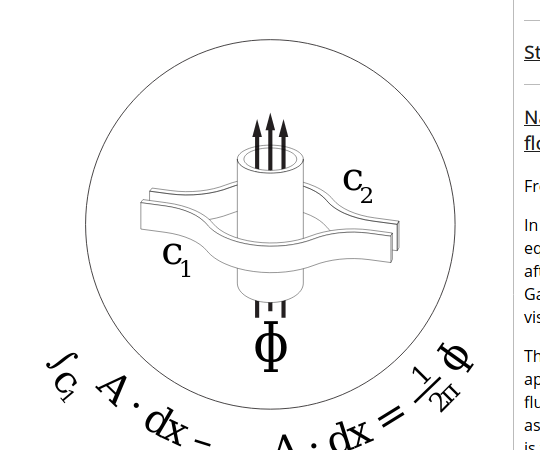
\includegraphics[width=0.20\linewidth]{./abohm.png}
    \end{center}
  \end{equation1}

  \begin{equation1}[Yang-Baxter Equation]
    $\;$
    \newline
    \begin{center}
      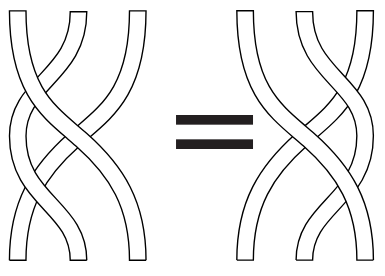
\includegraphics[width=0.15\linewidth]{./yang-baxter.png}
    \end{center}
  \end{equation1}

  \begin{equation1}[Euler Characteristic]
    $$ \chi = V - E + F $$
  \end{equation1}

  \begin{equation1}[Gauss-Bonnet]
    $$2\pi \chi = \int_M K dA$$
  \end{equation1}


	\begin{equation1}[Stoke's Theorem]
    $$\int_M d\omega = \int_{\partial M} \omega $$
  \end{equation1}

  \begin{equation1}[Dirac Equation]
    $$(i{\partial\!\!\!\big /} - m) \psi = 0$$
  \end{equation1}

  \begin{equation1}[Heisenberg]
    $$[Q(f), Q(g)] = i\hbar Q(\{f,g\})$$
  \end{equation1}

  \begin{equation1}[Levi Cicita]
    $$\nabla g = 0,\nabla_X Y - \nabla_Y X = [X,Y]$$
  \end{equation1}

  \begin{equation1}[Klein Gordon]
    $$\Box \psi + \partial_{\psi}V = 0$$
  \end{equation1}

  \begin{equation1}[Borel-Weil-Bott]
    $$\forall i : H^i(G/B,L_\lambda) = 0$$
  \end{equation1}

  \begin{equation1}[Einstein Field Equations]
    $$R_{\mu\nu} - \frac{1}{2}Rg_{\mu\nu} + \Lambda g_{\mu\nu} = \frac{8\pi G}{c^4}T_{\mu\nu}$$
    \begin{center}
      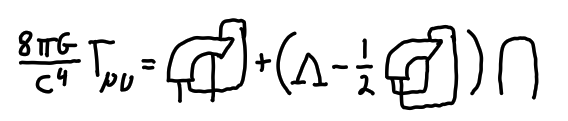
\includegraphics[width=0.30\linewidth]{./einf.png}
    \end{center}
  \end{equation1}

  \begin{equation1}[Riemann Curvature Tensor Decomposition]
    $$S_{abcd} + E_{abcd} + C_{abcd}$$
    \begin{center}
      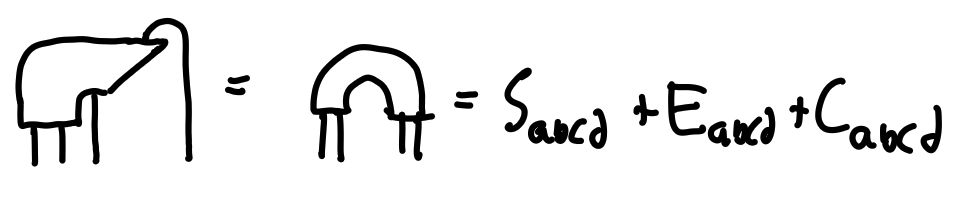
\includegraphics[width=0.30\linewidth]{./decomp.png}
    \end{center}
  \end{equation1}

  \begin{equation1}[Bianchi Identity]
    $\;$
    \newline
    \begin{center}
      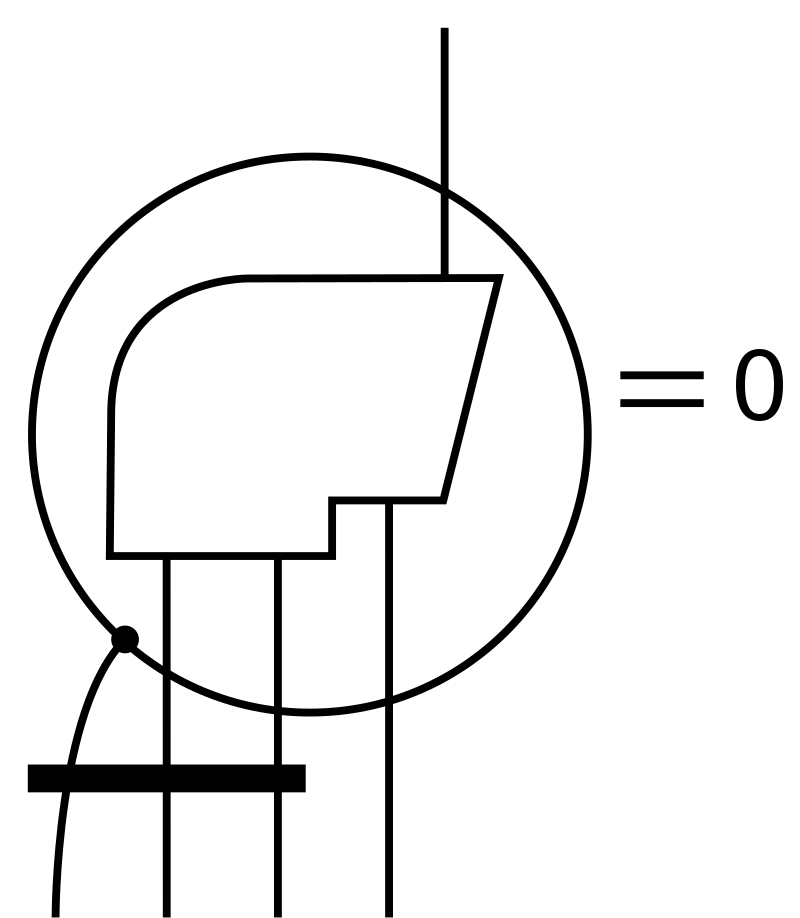
\includegraphics[width=0.15\linewidth]{./bianchi.png}
    \end{center}
  \end{equation1}

  \begin{equation1}[Energy-Mass Equivalence]
    $$E = \gamma mc^2 $$
  \end{equation1}

  \begin{equation1}[Faraday Tensor]
    $$F = dA$$
  \end{equation1}

\end{section}

\begin{section}{Rough Equations}

  \begin{equation1}[Bianchi to Maxwell]
    $F =dA$
    \newline $df = d^2A = 0$
    \newline $\nabla[_{\alpha}F_{\beta\gamma}] = 0$
    \newline $J \star F = \mu_0J$
    \newline $\Rightarrow \partial_{\alpha}F^{\alpha \beta} = \mu_0 J^{\beta}$
  \end{equation1}

  \begin{equation1}[Yang-Mills Equations]
    $$\langle s,t \rangle_{L^2} = \int_X \langle s,t \rangle dvol_g$$ $$ \langle d_A s,t \rangle_{L^2} = \langle s, d^*_A t\rangle_{L^2}$$ $$d^*_A F_A = 0$$ $$d_A \star F_A = 0$$ $$d\omega = d^*\omega = 0$$
  \end{equation1}

  \begin{section}{Legacy Equations}

    \begin{equation1}[Bianchi Identity]
      $R^{h}_{ijk,l} + R^{h}_{ikl,j} + R^{h}_{ilj,k} = 0$
      \newline or
      \newline $D\Theta = \Omega \land \theta$ and $D\Omega = 0$
    \end{equation1}

    \begin{equation1}[Faraday Tensor]
      $dA = F$
    \end{equation1}

    \begin{equation1}[Energy-Mass Equivalence]
      $E_r = \sqrt{(m_0c^2 )^2 + (pc)^2}$
    \end{equation1}

  \end{section}

  \begin{equation1}[Riemann Curvature Tensor Decomposition]
    $R_{abcd} = S_{abcd} + E_{abcd} + C_{abcd}$

  \end{equation1}

  \begin{equation1}[Klein Gordon]
    $\square \psi + \partial_{\psi}V = 0$
  \end{equation1}
  
  \begin{equation1}[Dirac Equation]
    $$\Big(\beta mc^2 + c\sum^{3}_{n=1}\alpha p_n \Big)\psi(x,t) = i\hbar \partial_t \psi(x,t)$$
  \end{equation1}

  \begin{equation1}[Yang-Baxter Equation]
    $$ ( \widecheck{R} \otimes 1)(1 \otimes \widecheck{R})(\widecheck{R} \otimes 1) = (1 \otimes \widecheck{R})(\widecheck{R} \otimes 1)(1 \otimes \widecheck{R})$$
  \end{equation1}

  \begin{equation1}[Supergravity Lagrangian]
    $$\mathscr{L} = R - \psi^-_\mu \upgamma^{\mu \rho \sigma}D_\rho \psi_{\sigma}$$
  \end{equation1}

  \begin{equation1}[Atiyah-Singer]
    $$\ind{D_e} = \dim \ker D_E - \dim \ker D_E^* = \int_M \hat A(M,g) \text{ch}^{E/\mathbb{S}}(E/\mathbb{S}) $$
  \end{equation1}

  \begin{equation1}[Maxwell]
    $dF  = 0$
    \newline $d \star F = J$
  \end{equation1}

\end{section}
\end{document}
